\section{Overview} \label{sec:design}
	\noindent For means of explanation, the architecture of the FPGA based implemented DRFM system can be described by three subsystems. These being, the interfacing and control system, the external peripherals and the DSP system. Whereby each of the constituent systems are monitored and controlled by the top-level controller module. This simplified architecture may be seen in Fig.~\ref{fig:DRFM_Architecture}.\\ \newline It must be noted that the architecture described in Fig.~\ref{fig:DRFM_Architecture} has not yet been integrated into a RF front end and therefore this paper is a review of the work in progress. The implications of this are that although real time signal processing and data storage are realizable at the speeds dictated by the RF front-end, it has not been proven that it is possible using this design. 
	\begin{figure*}[h!]
		\centering
		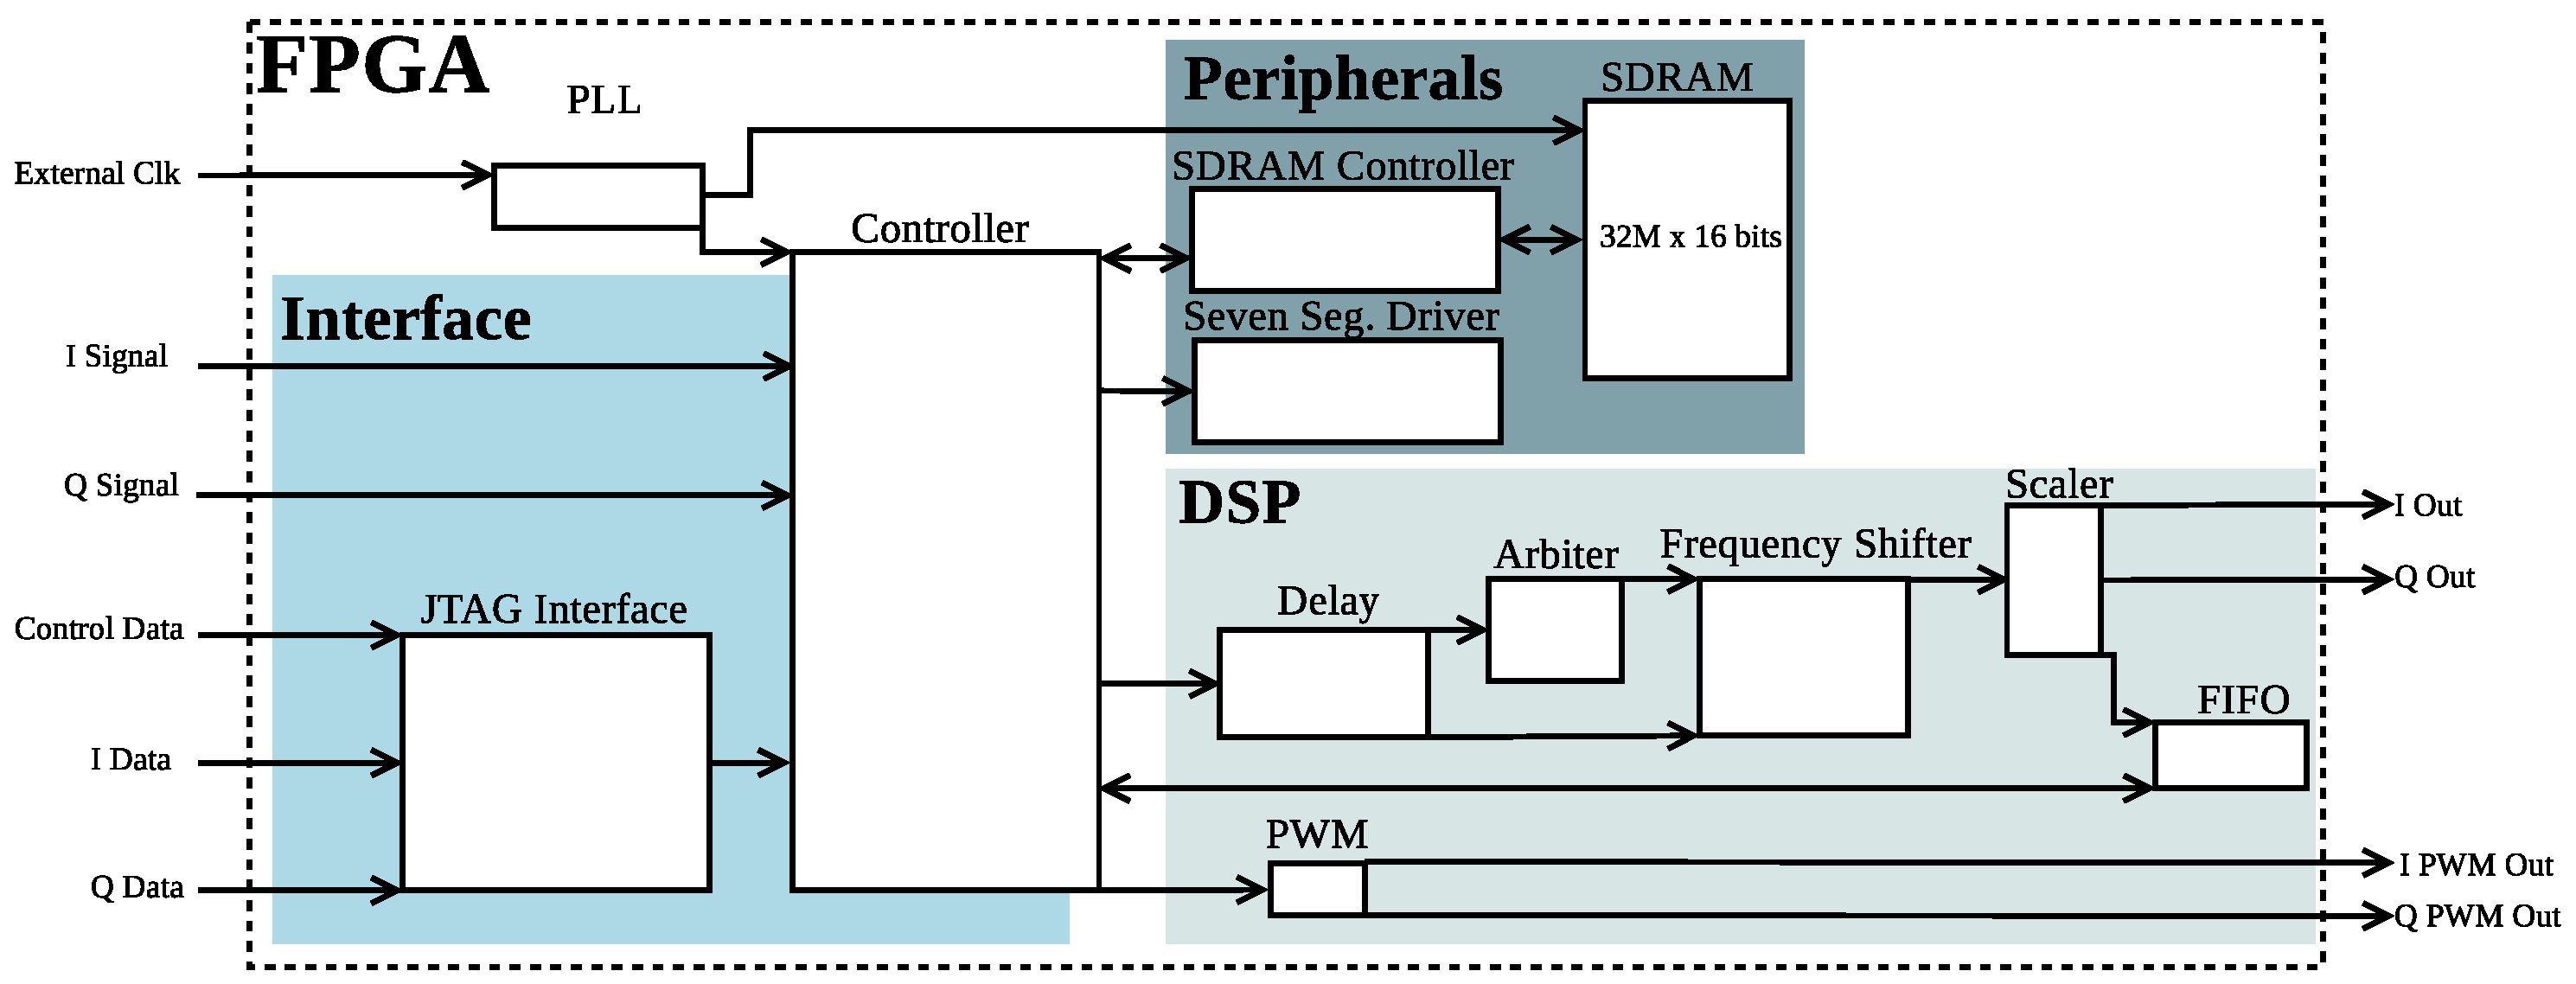
\includegraphics[width=0.95\linewidth]{img/System_Overview}
		\caption{Illustration of the implementation of the  FPGA based DRFM System}
		\label{fig:DRFM_Architecture}
	\end{figure*}
	
	\subsection{Interface}
		\subsubsection{JTAG Interface}
		 Joint Action Test Group (JTAG) was originally used as a simplified standard for interconnectivity testing for PCB manufacturing. It was created as a result of Integrated Circuits (IC) pins becoming more densely spaced and therefore classical interconnectivity test approaches were infeasible. The JTAG protocol mitigated the need for physical access to an IC's pins through the use of shift register chains.  \\ \newline In the JTAG standard (IEEE 1149.1) the collections of shift registers are referred to as Boundary Scan Cells (BSCs) which sample and hold data from and to the pin interface. As a result the BSCs can be configured into a serial shift chain thereby allowing to be driven by a serial interface. \\ \newline 	The JTAG interface implemented on the DRFM system allows for software based monitoring, updating and controlling of the DRFM system through the JTAG port.  Through the use of the Altera Virtual JTAG Intellectual Property (IP) core it is possible to access to the JTAG control signals that are routed to the FPGA core. This allows for a fine control over the JTAG resources thereby granting real-time general purpose serial communication \cite{JTAG}. \\ 
		\subsubsection{User Interface}
		Through the use of  a Python  based User Interface (UI) that runs a TCL JTAG server it is possible to transfer both I/Q data as well as control information to the FPGA as may be seen in Fig.~\ref{fig:DRFM_Architecture}. The control word consists of 64 bits with flags and data contained within its length. The control word composition may be seen in Table.~\ref{tab:Control_Info} given that the most significant bit is at position 61.
		
		\begin{table}[h!]
			\centering
			\caption{Control Word Composition}
			\begin{tabular}{ccc}

				\textbf{Control Information} & \textbf{Control Flag Position} & \textbf{Control Data Length} \\ 
				Doppler Shift 	& 33 & 32  \\
				Time Delay    	& 44 & 10 \\
				Amplitude Scale & 61 & 16 
			\end{tabular}
		\label{tab:Control_Info}
		\end{table}
		\noindent In addition to this, the UI was capable of transferring 32 bits of I/Q data via JTAG to the FPGA system on demand. Where the I/Q data were 16 bits wide respectively. 
	
	\subsection{External Peripherals}
	\noindent In order to account for the requirement of I/Q data injection, an external SDRAM memory was incorporated into the DRFM system. It was used as a means to store the injected I/Q data so that it could be recalled for the DSP operations of the DRFM system. The SDRAM device is a 512Mb high speed CMOS dynamic access memory with 32M of address space that address 16 bit words \cite{SDRAM}. \\ \newline Due to the fact that each I/Q channel were 16 bits wide, it was necessary to interleave the I/Q data samples. Where the first address contained I data and the next Q data. \\ \newline A SDRAM controller was implemented on the FPGA in order to facilitate communication with the external SDRAM peripheral. The controller made use of the Altera SDRAM Controller IP Core which uses the Avalon Interfacing standard to communicate with the SDRAM device. This was integrated into the system through the use of the Altera Qsys tool, that allowed for pin allocations to the external SDRAM device \cite{SDRAM_Core}. \\ \newline In addition to this it was required to clock the external SDRAM device at different clock rate. Therefore it was necessary to implement a Phase Locked Loop (PLL) in order to synchronously  step down the clock speed.\\ \newline Finally, for debugging and user interfacing purposes a group seven segment displays were used. The seven segment displays gave visual feedback to the operator of the system by displaying the current state of the DRFM system.
	\subsection{Digital Signal Processing}
	\noindent As previously discussed, the digital signal processing aspect of a DRFM system was critical to its operation. As time delays, frequency shifts and amplitude scalings were needed in order to emulate a target from a radar system's perspective. \\ \newline The major consideration in the implementation of this signal processing scheme was the order in which the signal processing operations were performed. This was due to the real-time processing requirements of a DRFM system, such when performing variable time delays there would be no loss of coherence between the input and output signals. \\ \newline  This meant that if a time delay was set by the user and a frequency shift was then applied, the system should not have to repopulate the delay buffer. For this reason the order of the signal processing operations were to first perform the time-delay, then frequency shifts and finally amplitude scaling, as can be seen in Fig.~\ref{fig:DRFM_Architecture}.\\   \subsubsection{Signal Processing Model}In order to describe the signal processing model, the signal, $s_{rx}(n)$, is considered to be the input to the signal processing chain. As the DRFM system receives I/Q data, $s_{rx}(n)$ may be  expressed mathematically as
	\begin{equation}
		s_{rx}(n) = v_{rx}(n) +j\hil \{v_{rx}(n)\} = I(n) +jQ(n)
	\end{equation}
	\noindent where $v_{rx}(n)$ is the digitized received RF signal and $\hil \{v_{rx}(n)\}$ is the Hilbert Transform of $v_{rx}(n)$. Such that, $v_{rx}(n)$ is equal to $I$ and $j\hil \{v_{rx}(n)\}$ is equal to $jQ$.  \\ \newline This model is used as it lends itself to the analytic signal representation of the incoming RF signal. This being that the I/Q data does not contain any negative frequency components. As the $I$ component is a replica of the incoming RF signal and the $Q$ component is a $90^\circ$ phase shifted version of the RF signal, thereby resulting in their sum yielding no negative frequency components. The benefit of this is that it allows one to sample at the RF frequency, rather than at the Nyquist Rate and that it simplifies the arithmetic operations applied to these signals. \cite{wil} \\
	\subsubsection{Time Delay}
	 The time delay operation may be expressed as a method of altering the index of the input signal $s(t)$. This process may be summarized mathematically by
	\begin{equation}
		s_{delay}(k) = s_{rx}(n -k),\quad n \geq k.
	\end{equation}
	 \noindent This model may be implemented on a digital system by injecting a portion of the input signal $s_{rx}(n)$ into a RAM. After which, indexing previous values of $s_{rx}(n)$ by means of the RAM's address pointers. Which then allows for the outputting of previous values of the inputted signal given that capacity criteria has been met. This being that the delay address index, $k$, is less than or equal to current RAM address index, $n$. In the implementation of the DRFM system, a dual port, 1024 address long, 16 bit wide RAM is implemented internally on the FPGA. \\
	\subsubsection{Frequency shifting}
	The frequency shifting model implemented on the DRFM system can be easily summarised mathematically by the following expression 
	\begin{equation}
		s_{s}(n) = s_{rx}(n) e^{j2\pi f_{s}n}
	\end{equation} 
	\noindent where $s_{s}(n)$ is the shifted version of $s_{rx}(n)$ and $f_s$ is the shift frequency. By expanding the complex exponential term into its constituent sinusoids and using the previously explained I/Q signal model it can be seen that
	\begin{equation}
	\label{eq:shift}
		\begin{split}
			s_{s}(n) &= [I(n) +jQ(n)][cos(2\pi f_{s}n) +jsin(2\pi f_{s}n)] \\
			         &=  [I(n)cos(2\pi f_{s}n) - Q(n)sin(2\pi f_{s}n)] \\
			         &\quad+j[I(n)sin(2\pi f_{s}n) +Q(n)cos(2\pi f_{s}n)]\\
			         &= I_s(n) +jQ_s(n)
		\end{split}
	\end{equation}
	\noindent where $I_s(n)$ can be considered to be the real frequency shifted component and $jQ_s(n)$ is the complex frequency shifted component. \\ \newline The implications of Equation.~\ref{eq:shift} are that the frequency shifter can be implemented through the use of four multipliers, an addition and a subtraction.\\ 
	
	\subsubsection{Amplitude Scaling}
		As control word allocates 16 bits to the amplitude scaling information, a model was implemented to translate the control data to a value between 1 and 0. This was achieved by applying a non circular bit shift to the amplitude scaling portion of the control word. Such that the amplitude scaling information would be shifted 16 bits to the right in order to scale it between 1 and close to zero. This operation may be expressed mathematically by
		\begin{equation}
			s_{scaled} (n) = 2^{-p} A \; s_{rx}(n),\quad 0 \leq p \leq 15
		\end{equation}
		where $p$ is the number of shifted positions the amplitude scaling section of the control word is shifted by and $A$ is the magnitude of the amplitude control word. This is possible due to the properties of the binary number system as shifting a bit sequence right by one position implies a division by 2. \\ \newline The implications of this are that the smallest number that can be represented is $30.52\times10^{-6}$, which for the practicalities of this system is sufficient as a DRFM should not have to attenuate the outputted signal completely.\\
		
	\subsubsection{Complete Signal Model}
	From the above derivations it is possible to conclude that the outputted signal  can be expressed mathematically by
	\begin{equation}
		s_{tx} (k) = 2^{-p} A\; s_{rx}(n -k) e^{j2\pi f_{s}n}.
	\end{equation}
		
	
	



